\documentclass{article}

\usepackage{neurips_2019_author_response}

\usepackage[utf8]{inputenc} % allow utf-8 input
\usepackage[T1]{fontenc}    % use 8-bit T1 fonts
\usepackage{hyperref}       % hyperlinks
\usepackage{url}            % simple URL typesetting
\usepackage{booktabs}       % professional-quality tables
\usepackage{amsfonts}       % blackboard math symbols
\usepackage{nicefrac}       % compact symbols for 1/2, etc.
\usepackage{microtype}      % microtypography

\usepackage{amsmath}
\usepackage{amssymb}
\usepackage{bm}

\usepackage{wrapfig}

\usepackage{tikz}

\usetikzlibrary{shapes,arrows}

\tikzstyle{block} = [rectangle, draw, thick, align=center, rounded corners]
\tikzstyle{boundingbox} = [very thick, dotted, gray]
\tikzstyle{dashblock} = [rectangle, draw, thick, align=center, dashed]
\tikzstyle{conc} = [ellipse, draw, thick, dashed, align=center]
\tikzstyle{netnode} = [circle, draw, very thick, inner sep=0pt, minimum size=0.5cm]
\tikzstyle{relunode} = [rectangle, draw, very thick, inner sep=0pt, minimum size=0.5cm]
\tikzstyle{line} = [draw, very thick, -latex']
\tikzstyle{arrow} = [draw, ->, very thick]

\begin{document}
\begin{wrapfigure}{r}{0.27\textwidth}
\begin{center}
\vspace{-0.85em}
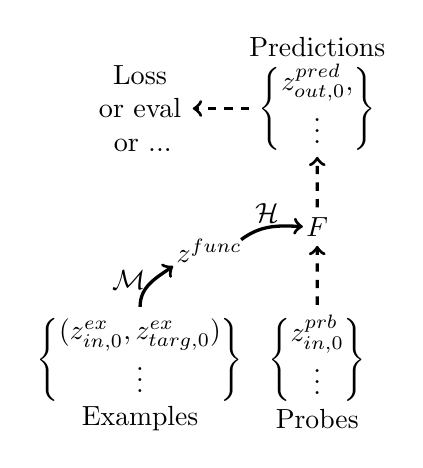
\begin{tikzpicture}[auto, scale=0.75]
\node at (-1.5, -3.5) (examples) {Examples};
\node at (-1.5, -2.5) (D1) {
\(\left\{
\begin{matrix}
(z^{ex}_{in,0}, z^{ex}_{targ,0})\\
$\vdots$
\end{matrix}\right\}\)};

\node at (1.5, -3.5) (examples) {Probes};
\node at (1.5, -2.5) (D2) {
%\(z^{prb}_{in}\)};
\(\left\{
\begin{matrix}
z^{prb}_{in,0}\\
$\vdots$
\end{matrix}\right\}\)};

\node at (-0.33, -0.66) (zfunc) {\(z^{func}\)};

\path [arrow] (D1) to [in=-145, out=90] ([xshift=3, yshift=3]zfunc.south west) node [xshift=-16, yshift=-5] {\(\mathcal{M}\)};

\node at (1.5, -0.25) (F) {\(F\)};

\path [arrow, bend left] ([xshift=-5, yshift=-5]zfunc.north east) to [in=165, out=25] ([xshift=3]F.west) node [xshift=-13, yshift=5]{\(\mathcal{H}\)};

\path [arrow, dashed] (D2) to (F);

\node at (1.5, 1.75) (outputs) {
%\(z^{pred}_{out}\)};
\(\left\{
\begin{matrix}
z^{pred}_{out,0},\\
$\vdots$
\end{matrix}\right\}\)};
\node at (1.5, 2.8) (predictions) {Predictions};

\path [arrow, dashed] (F) to ([yshift=3]outputs.south);

\node [align=center, text width=1.25 cm] at (-1.5, 1.75) (dispatch) {Loss or eval or ...};

\path [arrow, dashed] (outputs.west) to ([xshift=-3]dispatch.east);
\end{tikzpicture}
\end{center}
\vspace{-2.3em}
\end{wrapfigure}
\looseness=-1
We thank the reviewers for their thoughtful and thorough reviews. \par
\looseness=-1
\textbf{Architecture \& contributions:} We agree with the reviewers that the most novel contribution of our paper is the proposal to think about transfer in terms of meta-mappings and task transformations. We would like to clarify the architecture and training. First we will clarify how a basic polynomial is learned. This is depicted schematically on the right. As in standard meta-learning, we generate a set of examples, consisting of tuples of input point, and the target output (i.e. the polynomial evaluated at that point). The meta-network $\mathcal{M}$ processes this set of (embedded input, embedded target) pairs to produce a function embedding. Specifically, it concatenates each pair, applies two layers of identical processing to each concatenated pair independently, max pools elementwise across them, and then applies two more layers of processing to produce the function embedding $z^{func}$ for this polynomial. We pass the function embedding through the hyper network $\mathcal{H}$ to parameterize a function $F$ which performs the mapping from inputs to outputs. We can then use $F$ to transform a new set of probe inputs (i.e. points we want to evaluate the polynomial at) to produce a set of predictions, and then train or evaluate the model on corresponding targets. \par 
\looseness=-1
\textbf{The insight of our paper is that learning a meta-mapping over polynomials is exactly analogous to learning a polynomial.} Instead of having examples of inputs and outputs for a single polynomial, we have examples of input polynomials and output polynomials for the meta-mapping that operates over polynomials (e.g. multiplying by 2). Specifically, a set of polynomials are embedded as above, by passing examples of them through the meta network to compute a function embedding for each one. We then take a set of pairs of (embedded input polynomial, embedded target polynomial), and pass them through the \textbf{exact same meta network} $\mathcal{M}$ to produce an embedding for the function that transforms one polynomial into another. Just as above, we pass this function embedding through the same hyper network $\mathcal{H}$ to parameterize a function $F$ which attempts to multiply polynomials by 2. We can then pass a probe polynomial through $F$ to produce a predicted output. The only differences from the basic case are: 1) where the inputs and targets come from 2) how the loss or evaluation is computed from the predictions. For basic training, we used an appropriate loss in the output space for each task; in meta training, we used an $\ell^2$ between the predicted task embedding and the embedding of the target task. One of the main algorithmic insights of our work is that this produces $z^{func}$ embeddings which approximate the desired meta-mapping well, even for meta-mappings not included in training (see fig. 3). To evaluate meta-mapping performance, we actually computed the performance of the predicted output embedding at computing the target polynomial. For example, if the meta-mapping was ``multiply by 2'' and the probe input was the function embedding of $x + 2$, we would evaluate how closely the predicted output polynomial matched $2x + 4$, by feeding the predicted function embedding to the hyper network to parameterize a function, feeding input values to this function, and then measuring its predicted outputs against the real values of $2x+4$ at those inputs. We hope this clarifies our approach, and why it is fundamentally different from prior work. All three reviewers highlighted the novelty of considering transformations over tasks. That is the conceptual contribution of our paper, and the algorithmic contribution is to show an approach for solving this challenge. Notably, because we use the same networks for both basic tasks and meta-mappings, our approach is parsimonious --- it does not require adding any new parameters to the model. (We show in Appendix D.1 that this actually performs better than having separate meta and hyper networks for basic tasks and meta-mappings.) While other meta-learning approaches could potentially be adapted to do meta-mappings, it is unclear that they could be adapted so parsimoniously, or perform well. However, we think exploring alternate approaches, or combining algorithms like MAML with architectures like ours, provide exciting future directions. For now, we are revising the main text to clarify our message. \par 
\looseness=-1
\textbf{Architecture:} The reviewers noted that some of the architectural choices seemed arbitrary. We justify some choices in appendix D, but we acknowledge that we have not explored the full space of approaches to this problem, this will be important future work. On the DQN: the problem is not exactly a standard supervised problem because you have multiple betting actions and only observe the reward for the bet you execute, we have clarified this in the text. \par 
%\textbf{Relation to other work:} We do think that combining other meta-learning approaches such as MAML with a system like ours is an interesting direction for future work. \par 
%\looseness=-1
%\textbf{Contributions:} As all three reviewers noted, the most novel contribution of our paper is the proposal to think about transfer in terms of meta-mappings and task transformations. The architecture we propose is designed with this idea in mind. It is true that previous work has considered task embeddings (some of the works suggested by the reviewers we have mentioned in the related works section, but some we were not familiar with, we appreciate the pointers). Most of this work has developed some way of embedding a task or dataset into some latent space. However, what we think is fundamentally novel about our architecture is that \textbf{we use the same latent space for the dataset as we use for an individual input to the network}. This allows us to use the same meta and hyper networks for both basic tasks and meta-mappings. We show in appendix D.1 that this performs better than separate embedding spaces. We think that this is a fundamentally novel aspect of our architecture, since it is primarily useful for the meta-mappings we propose. While other techniques that create explicit task embeddings could also be trained to transform them for meta-mappings, we think our novel insight of a shared embedding space for individual data points and tasks would result in better performance with other algorithms too. We do think that combining other meta-learning approaches such as MAML with a system like ours is an interesting direction for future work. As we point out in the future directions, we do not expect the exact approach we've proposed to be the best way of solving these problems. However, it does provide a useful starting point. We think that the primary contribution of this work is highlighting the idea of meta-mappings for transfer, and providing some starting points for how to approach them by taking a functional perspective, which we hope will inspire future work. \par
%\looseness=-1
%\textbf{Meta-mapping details:} For a concrete training example, imagine trying to map from winning tasks to losing them. Suppose we have three tasks, chess, poker, and go, and losing variations of each. We generate task embeddings for each game, e.g. $z_{poker}$, by applying the meta network $\mathcal{M}$ to experiences from the game. We randomly select some games (poker, go) to use as training examples to generate the meta-mapping parameters, and hold-out the rest (chess) to make the generated meta-mapping generalize. We thus generate a dataset $D = {(z_{poker}, z_{lose-poker}), (z_{go}, z_{lose-go})}$. Per above, we process this dataset using the same meta-network $\mathcal{M}$ to get a function embedding $z_{lose} = \mathcal{M}(D)$ for the meta-mapping. We can then pass this embedding through the hypernetwork $\mathcal{H}$ in order to parameterize a mapping $F_{z_lose}$ which attempts to map game strategies to strategies for the losing variation of that game. We use this mapping to transform each input embedding and compute the $\ell_2$ loss between the result and the target function embedding, e.g. for chess the loss would be $(F_{z_lose}(z_{chess}) - z_{lose-chess})^2$. We minimize this loss across all held-out and training examples (using both accelerates learning). We then proceed with the next meta-mapping. \par
%\looseness=-1
%To evaluate performance on a meta-mapping, we generate the training dataset as above, but we do not assume we have an embedding for the held-out targets. For example, we may know how to play chess via a task embedding $z_{chess}$, but our goal is to figure how to lose at chess. So we take $\hat{z}_{lose-chess} = F_{z_{lose}}(z_{chess})$, and use it to play losing chess by parameterizing a function $F_{\hat{z}_{lose-chess}}$. We then evaluate this function's actual performance on losing chess, which tells us the true quality of the meta-mapping. We hope this clarifies the training and evaluation of meta-mappings. We have revised the manuscript to be more explicit about this and fix typos noted by reviewer 1, and if our manuscript is accepted we will also incorporate more details of tasks and training from the appendix as space allows. \par
\looseness=-1
\textbf{miniImageNet:} We didn't have time to evaluate on all the requested datasets, but on miniImageNet, using a ResNet-50 as the input encoder, we achieved test accuracy of 61.0\% on 5-shot, 5-way classification, competitive with e.g. MAML. We expect that with more than a few days to tune hyperparameters and train larger models we could do much better. \par
\looseness=-1
\textbf{Datasets:} Our tasks will be released on github as stand-alone python modules that other researchers can use. \par
\looseness=-1
\textbf{Language \& continual learning:} In the revised paper we will emphasize the main points before discussing these extensions. We wanted to include language because it provides a simpler way to cue meta-mappings. Specifically, we used the language embedding as input to $\mathcal{H}$ instead of using examples via $\mathcal{M}$. For continual learning, while approaches like LEO generate (and even optimize) task embeddings, we are not aware of prior work that describes the continual learning approach of optimizing only the cached embeddings. Approaches like EWC double the parameter count by adding an ``importance'' parameter for each model parameter. For modern models with up to billions of parameters, caching a relatively low-dimensional task embedding instead could require less memory even up to millions of tasks. 
\end{document}
